\documentclass[aspectratio=169]{beamer}

\usepackage[utf8]{inputenc}
\usepackage{array}
\usepackage{booktabs}
\usepackage{bold-extra}
\usepackage{graphics}
\usepackage{hyperref}
\hypersetup{%
  colorlinks=true,
  linkcolor=blue,
  filecolor=blue,
  urlcolor=cyan,
}
\usepackage{listings}
\usepackage{multicol}
\usepackage[absolute,overlay]{textpos}
\usepackage{setspace}
\usepackage{verbatim}
\usepackage{fancyvrb} % for verbatim centering

\usetheme{Warsaw}
\usecolortheme{beaver}
\definecolor{clOrange}{HTML}{E76600}
\definecolor{clAlmostWhite}{HTML}{FEFFD9}
\definecolor{clGreen}{HTML}{007F00}
\definecolor{clFlag}{HTML}{D33682}
\definecolor{clFlagOpt}{HTML}{CB4B16}
\definecolor{clRedFlag}{HTML}{DC322F}
\definecolor{clViolet}{HTML}{4c0070}

\definecolor{clCodeBlue}{rgb}{0.0, 0.18, 0.38}
\definecolor{clCodeGreen}{rgb}{0.0, 0.27, 0.15}
\definecolor{clCodeRed}{rgb}{0.63, 0.0, 0.0}

\title[LTN07 :: cairographics]{Using cairo library to create PDF files}
\author{Adam Graliński}
\date[FFFE\_21]{\textbf{C++ {\color{red}F}{\color{blue}F}{\color{green}F}{\color{yellow}E}, May 2021}}

\setbeamertemplate{navigation symbols}{}
\setbeamercolor{title}{fg=black}
\setbeamercolor{author}{fg=clAlmostWhite}
\setbeamercolor{date}{fg=clAlmostWhite}
\setbeamerfont{author}{size=\huge}
\setbeamerfont{date}{size=\Large}

\newcommand{\greenemph}[1]{\textit{\textcolor{clGreen}{#1}}}
\newcommand{\cppmethod}[1]{\texttt{\textbf{\textcolor{clCodeBlue}{#1}}}}

\lstset{
  language=C++,
  basicstyle=\ttfamily,
  keywordstyle=\color{clCodeBlue}\ttfamily,
  stringstyle=\color{clCodeGreen}\ttfamily,
  commentstyle=\color{clCodeRed}\ttfamily,
  morecomment=[l][\color{magenta}]{\#}
}

\begin{document}

{\usebackgroundtemplate{%
 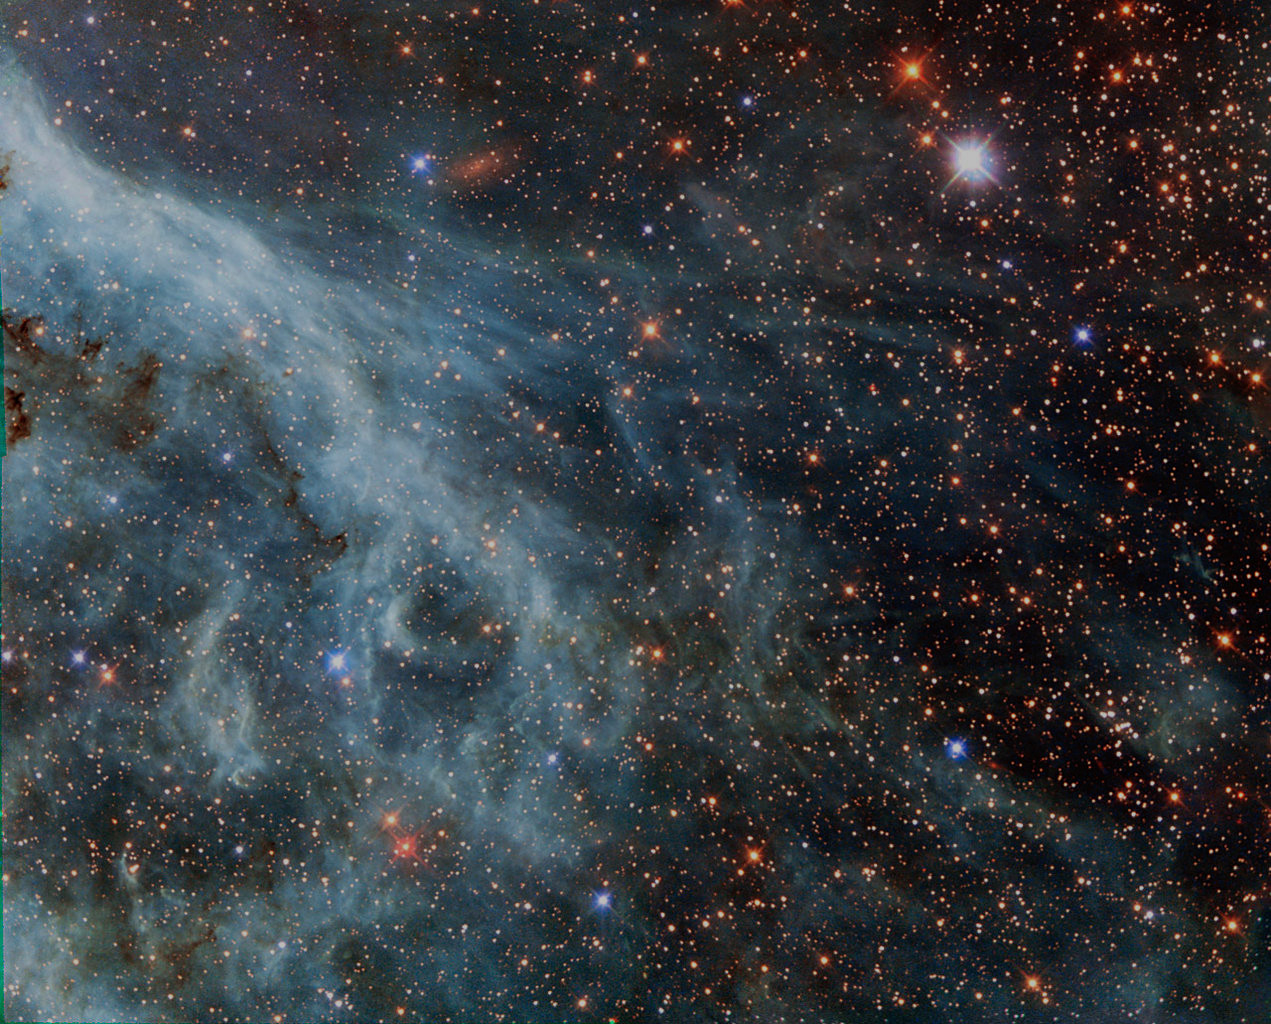
\includegraphics[width=\paperwidth,height=\paperheight]{../common/bg_galaxy.jpg}}
\begin{frame}
\titlepage{}
\end{frame}
}

\begin{frame}
\frametitle{Cairo}
{\centering

\includegraphics[width=4cm,keepaspectratio]{pics/CairoLogo.png}
\begin{itemize}
  \item open source 2D graphics library
  \begin{itemize}
    \item GNU Lesser General Public License (LGPL) 2.1 or Mozilla Public License (MPL) 1.1
  \end{itemize}
  \item support for multiple output devices
  \begin{itemize}
    {\tiny
    \item \greenemph{stable}: X Window System, Win32, image buffers, PostScript files, PDF files, SVGs
    \item \greenemph{experimental}: OpenGL, BeOS (Haiku), DirectFB
    }
  \end{itemize}
  \item provides subroutines for drawing primitives, stroking and filling, transforming, rendering text, etc.
  \item mature and stable project
  \begin{itemize}
    \item initial release before 2013
    \item latest release (\href{https://www.cairographics.org/news/cairo-1.17.4/}{1.17.4}) 29.11.2020,
          second-latest (\href{https://www.cairographics.org/news/cairo-1.17.2/}{1.17.2}) 01.02.2019,
  \item Written in C
  \end{itemize}
\end{itemize}
\hspace{4cm} \url{https://www.cairographics.org}
}
\end{frame}

\begin{frame}[fragile]
\frametitle{Simple usage}
\begin{columns}
  \begin{column}{0.3\textwidth}
    \begin{enumerate}
      \item create a drawing surface
      \item create cairo context
      \item stroke some curves, render some text, fill some polygon, etc.
      \item render the page
      \item destroy the allocated resources
    \end{enumerate}
  \end{column}
  \begin{column}{0.05\textwidth}
  \end{column}
  \begin{column}{0.65\textwidth}
    {\tiny
    \lstinputlisting[language=C++]{listings/01.cpp}
    \vspace{-12pt}
    \null\hfill{}Listing 1: creating an empty PDF page (\textit{listings/01.cpp})
    }
  \end{column}
\end{columns}
\end{frame}

\begin{frame}[fragile]
\frametitle{Sidenote: typographic points}
\begin{itemize}
  \item Cairo measures surfaces and primitives in \greenemph{typographic points}.
  \item in typography, 1 inch $=$ 72 tp
  \item use converting functions if you prefer metric system \\
{\tiny
\begin{lstlisting}[language=C++]
constexpr inline double mm_to_tp(double mm) { return mm / 25.4 * 72; }
\end{lstlisting}
}
  \item A4 page is 210$\times$297 millimeters wide.
\end{itemize}
\end{frame}

\begin{frame}[fragile]
\frametitle{Drawing a line}
{\large Let's draw \greenemph{a line}:}
\vspace{3mm}
  \begin{enumerate}
    \item set pen width\\
    \cppmethod{cairo\_set\_line\_width(cr, width);}\\
    \vspace{-5pt}
    {\tiny \url{https://www.cairographics.org/manual/cairo-cairo-t.html#cairo-set-line-width}}

    \item set pen color\\
    \cppmethod{cairo\_set\_source\_rgb(cr, red, green, blue);}\\
    \vspace{-5pt}
    {\tiny \url{https://www.cairographics.org/manual/cairo-cairo-t.html#cairo-set-source-rgb}}\\
    {\small note: the values for red, green and blue should be in range of [0.0 ... 1.0]}

    \item use \cppmethod{cairo\_move\_to(cr, x, y)} and \cppmethod{cairo\_line\_to(cr, x, y)} to draw a line\\
    \vspace{-5pt}
    {\tiny \url{https://www.cairographics.org/manual/cairo-Paths.html#cairo-move-to}}\\
    \vspace{-5pt}
    {\tiny \url{https://www.cairographics.org/manual/cairo-Paths.html#cairo-line-to}}

    \item finally call \cppmethod{cairo\_stroke(cr)} to stroke the path --- this draws the line\\
    \vspace{-5pt}
    {\tiny \url{https://www.cairographics.org/manual/cairo-cairo-t.html#cairo-stroke}}


  \end{enumerate}
\end{frame}

\begin{frame}[fragile]
\frametitle{Drawing a line}
\begin{columns}
  \begin{column}{0.7\textwidth}
    {\TINY
    \lstinputlisting[language=C++]{listings/02.cpp}
    \vspace{-12pt}
    }
    {\tiny \null\hfill{}Listing 2: drawing a blue line (\textit{listings/02.cpp})}
  \end{column}
  \begin{column}{0.3\textwidth}
    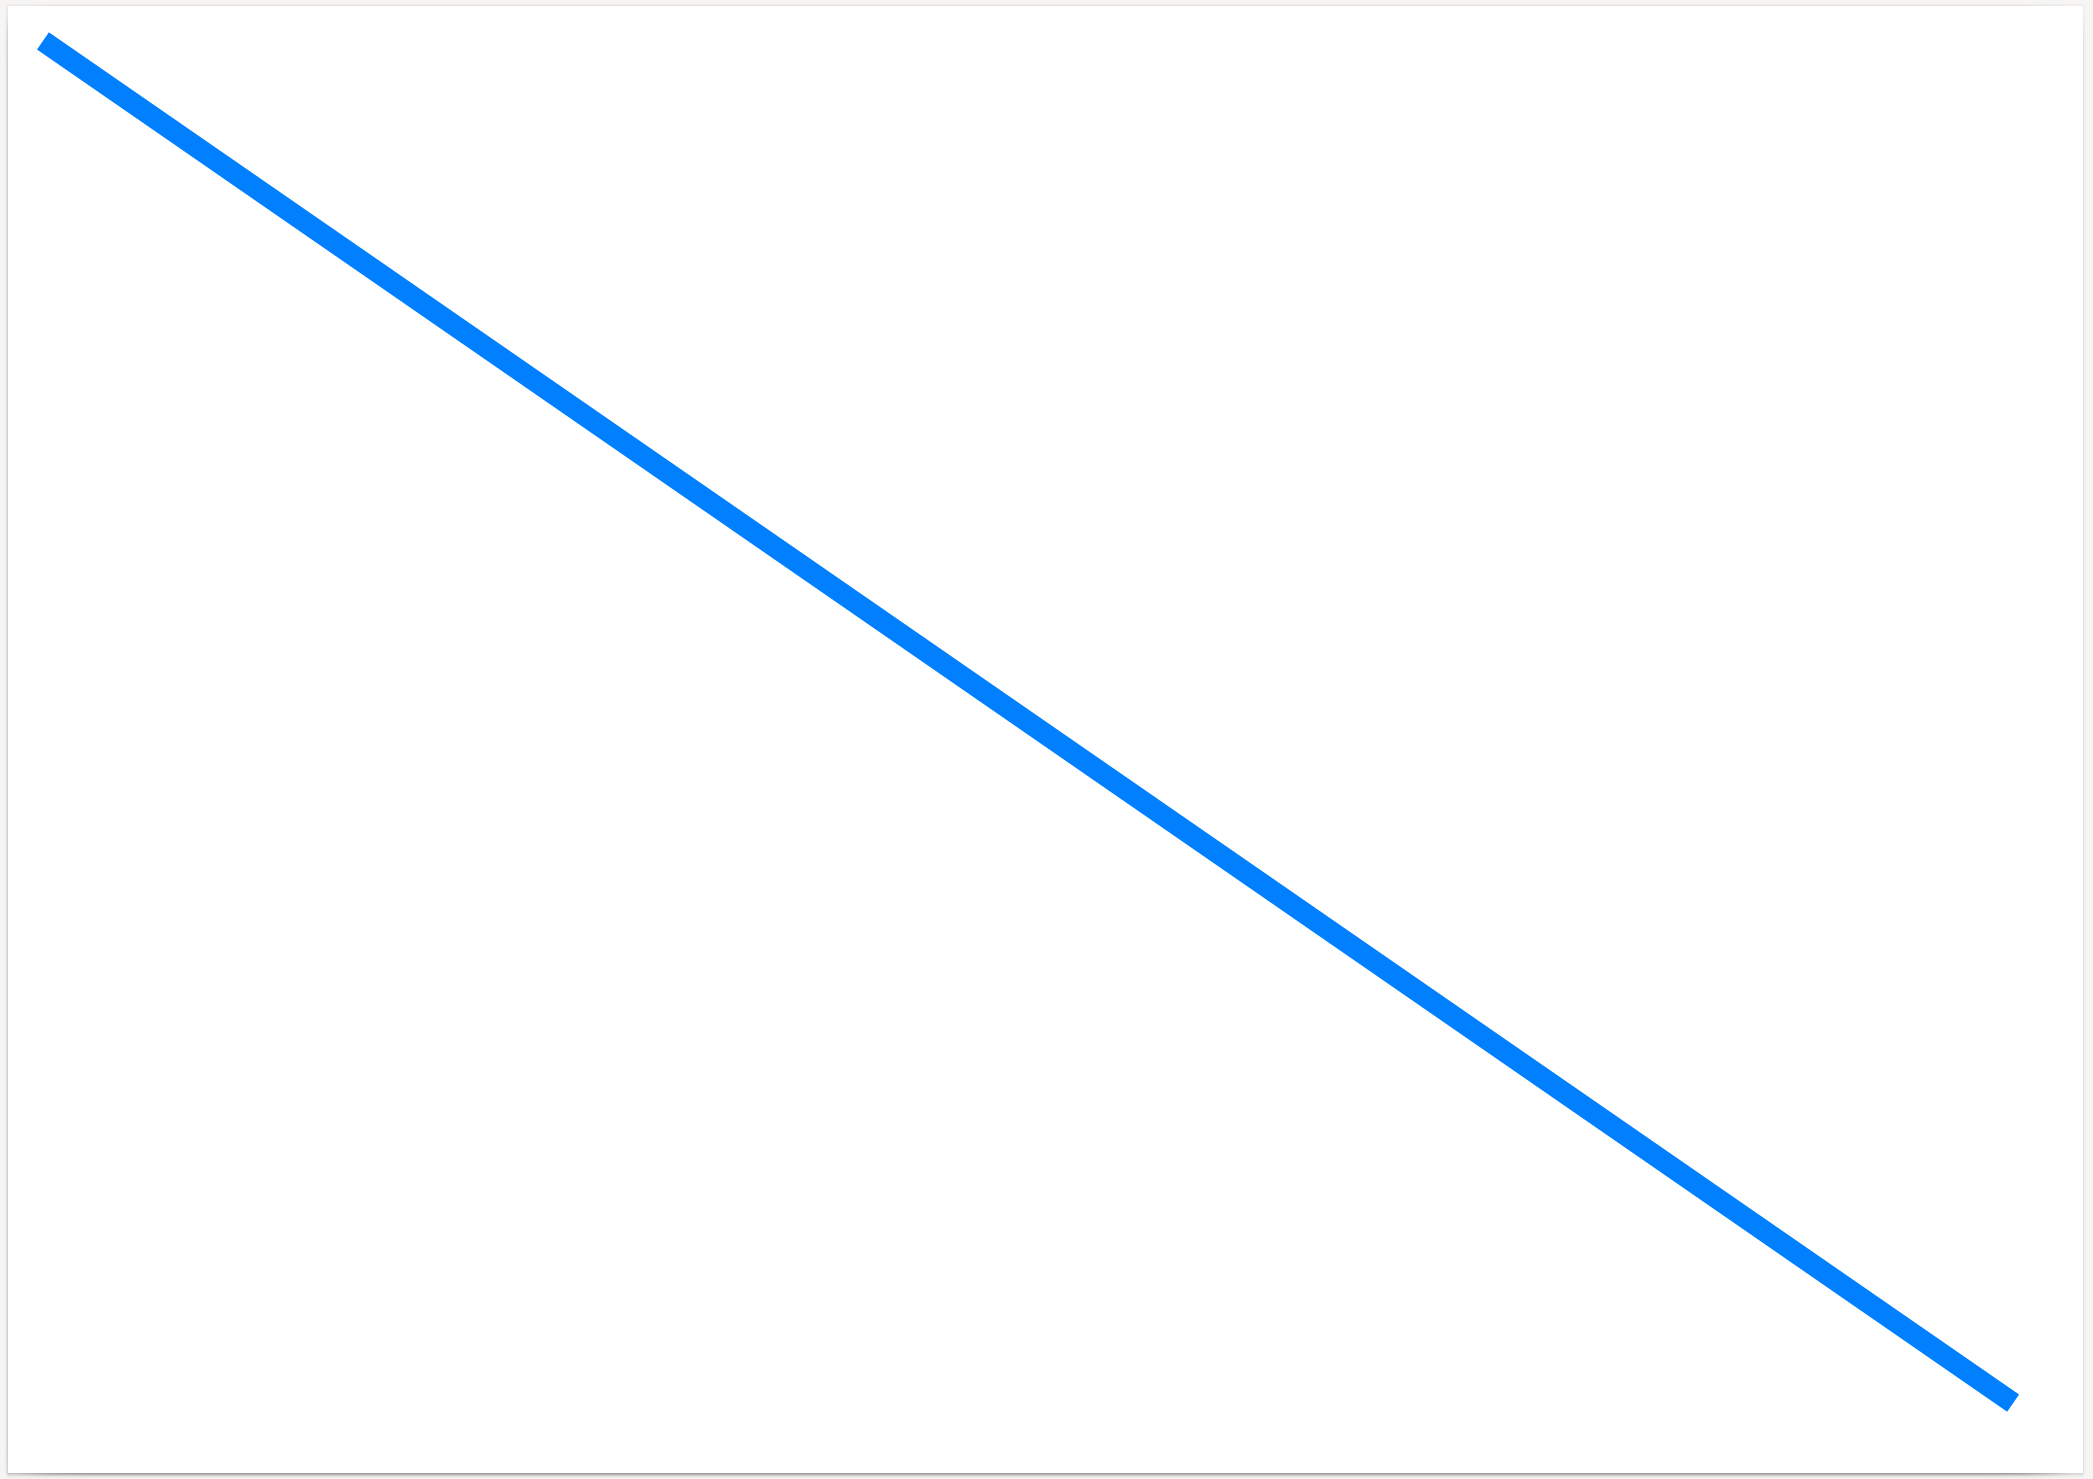
\includegraphics[width=4cm,keepaspectratio]{pics/output_02_line.png}
    \hspace*{24pt}{\small \textit{expected output}}
  \end{column}
\end{columns}
\end{frame}

\begin{frame}[fragile]
\frametitle{Drawing arcs and circles}
{\large Let's draw \greenemph{some circles}:}
\vspace{3mm}
  \begin{enumerate}
    \item set pen width\\
    \cppmethod{cairo\_set\_line\_width(cr, width);}\\
    \vspace{-5pt}
    {\tiny \url{https://www.cairographics.org/manual/cairo-cairo-t.html#cairo-set-line-width}}

    \item set pen color\\
    \cppmethod{cairo\_set\_source\_rgb(cr, red, green, blue);}\\
    \vspace{-5pt}
    {\tiny \url{https://www.cairographics.org/manual/cairo-cairo-t.html#cairo-set-source-rgb}}\\
    \vspace{-3pt}
    {\small note: the values for red, green and blue should be in range of [0.0 ... 1.0]}

    \item draw an arc\\
    {\small \cppmethod{cairo\_arc(cr, center\_x, center\_y, radius,  angle\_start, angle\_end)}}\\
    \vspace{-5pt}
    {\tiny \url{https://www.cairographics.org/manual/cairo-Paths.html#cairo-arc}}\\
    \vspace{-3pt}
    {\small note: angles are measured in radians}

    \item finally call \cppmethod{cairo\_stroke(cr)} to stroke the path --- this draws the arcs\\
    \vspace{-5pt}
    {\tiny \url{https://www.cairographics.org/manual/cairo-cairo-t.html#cairo-stroke}}
  \end{enumerate}
\end{frame}


\begin{frame}[fragile]
\frametitle{Drawing arcs and circles}
\begin{columns}
  \begin{column}{0.7\textwidth}
    {\fontsize{3pt}{2.7}\selectfont
    \lstinputlisting[language=C++]{listings/03.cpp}
    \vspace{-12pt}
    }
    {\tiny \null\hfill{}Listing 3: drawing colored arcs (\textit{listings/03.cpp})}
  \end{column}
  \begin{column}{0.3\textwidth}
    
\includegraphics[width=4cm,keepaspectratio]{pics/output_03_arcs.png}
    \hspace*{24pt}{\small \textit{expected output}}
  \end{column}
\end{columns}
\begin{textblock*}{\textwidth}(.5\textwidth,.9\textheight)
  \begin{beamercolorbox}[wd=.3\textwidth,left,sep=0.2cm]{listing}
    {\tiny Listing 3: drawing arcs (\textit{listings/03.cpp})}
  \end{beamercolorbox}
\end{textblock*}
\end{frame}


\begin{frame}[fragile]
\frametitle{Rendering text}
{\large Let's draw \greenemph{a caption}:}
\vspace{3mm}
  \begin{enumerate}
    \item set font face\\
    \cppmethod{cairo\_select\_font\_face(cr, font, slant, weight);}\\
    \vspace{-5pt}
    {\tiny \url{https://www.cairographics.org/manual/cairo-text.html#cairo-select-font-face}}

    \item set font size\\
    \cppmethod{cairo\_set\_font\_size(cr, size);}\\
    \vspace{-5pt}
    {\tiny \url{https://www.cairographics.org/manual/cairo-text.html#cairo-set-font-size}}\\
    \vspace{-3pt}

    \item move the pen to the chosen position\\
    \cppmethod{cairo\_move\_to(cr, x, y)}\\

    \item render the text\\
    \cppmethod{cairo\_show\_text(cr, text);}\\
    \vspace{-5pt}
    {\tiny \url{https://www.cairographics.org/manual/cairo-text.html#cairo-show-text}}
  \end{enumerate}
\end{frame}


\begin{frame}[fragile]
\frametitle{Rendering text}
\begin{columns}
  \begin{column}{0.7\textwidth}
    {\fontsize{3pt}{2.7}\selectfont
    \lstinputlisting[language=C++]{listings/04.cpp}
    \vspace{-12pt}
    }
  \end{column}
  \begin{column}{0.3\textwidth}
    
\includegraphics[width=4cm,keepaspectratio]{pics/output_04_text.png}
    \hspace*{24pt}{\small \textit{expected output}}
  \end{column}
\end{columns}
\begin{textblock*}{\textwidth}(.1\textwidth,.9\textheight)
  \begin{beamercolorbox}[wd=.5\textwidth,left,sep=0.2cm]{listing}
    {\tiny Listing 4: rendering a line of text (\textit{listings/04.cpp})}
  \end{beamercolorbox}
\end{textblock*}
\end{frame}


\begin{frame}
\frametitle{Real-life examples}
\begin{center}
  {\Large (demo)}
\end{center}
\end{frame}


\begin{frame}
\frametitle{Key takeaways}
{\centering
\begin{itemize}
  \item it's very easy to just get started with Cairo
  \item SVG images are supported too
  \item cairo text API is called a ``toy API'' for good reasons
  \begin{itemize}
    \item combine Cairo with Pango library if you need precise control over text rendering
  \end{itemize}
  \item use \href{https://www.cairographics.org/cairomm/}{cairomm} for full C++/STL support
  \item compile all listings with: {\tiny \cppmethod{g++ -std=c++20 `pkg-config --cflags --libs cairo` 0X.cpp}}
\end{itemize}

\vspace{2ex}
\begin{center}{\Large Thank you!}\end{center}
}
\end{frame}
\end{document}
